\documentclass[]{article}

\usepackage[left=2.00cm, right=2.00cm, top=2.00cm, bottom=2.00cm]{geometry}
\usepackage[spanish,es-noshorthands]{babel}
\usepackage[utf8]{inputenc} % para tildes y ñ
\usepackage{graphicx} % para las figuras
\usepackage{xcolor}
\usepackage{listings} % para el código fuente en c++

\lstdefinestyle{customc}{
  belowcaptionskip=1\baselineskip,
  breaklines=true,
  frame=single,
  xleftmargin=\parindent,
  language=C++,
  showstringspaces=false,
  basicstyle=\footnotesize\ttfamily,
  keywordstyle=\bfseries\color{green!40!black},
  commentstyle=\itshape\color{gray!40!gray},
  identifierstyle=\color{black},
  stringstyle=\color{orange},
}
\lstset{style=customc}

%opening
\title{Práctica 4. Exploración de grafos}
\author{David Luna Jurado \\ % mantenga las dos barras al final de la línea y este comentario
david.lunajurado@alum.uca.es\\ % mantenga las dos barras al final de la linea y este comentario
Teléfono: 663590384 \\ % mantenga las dos barras al final de la línea y este comentario
NIF: 32098835N \\ % mantenga las dos barras al final de la línea y este comentario
}


\begin{document}

\maketitle

%\begin{abstract}
%\end{abstract}

% Ejemplo de ecuación a trozos
%
%$f(i,j)=\left\{ 
%  \begin{array}{lcr}
%      i + j & si & i < j \\ % caso 1
%      i + 7 & si & i = 1 \\ % caso 2
%      2 & si & i \geq j     % caso 3
%  \end{array}
%\right.$

\begin{enumerate}
\item Comente el funcionamiento del algoritmo y describa las estructuras necesarias para llevar a cabo su implementación.

El valor de las celdas para la colocación del extractor de minerales se realiza calculando la distancia de dicha casilla respecto al centro.
El valor de la casilla será el inverso de la distancia, de esta forma las casillas más cercanas al centro tendrán más valor.

% Elimine los símbolos de tanto por ciento para descomentar las siguientes instrucciones e incluir una imagen en su respuesta. La mejor ubicación de la imagen será determinada por el compilador de Latex. No tiene por qué situarse a continuación en el fichero en formato pdf resultante.
\begin{figure}
\centering
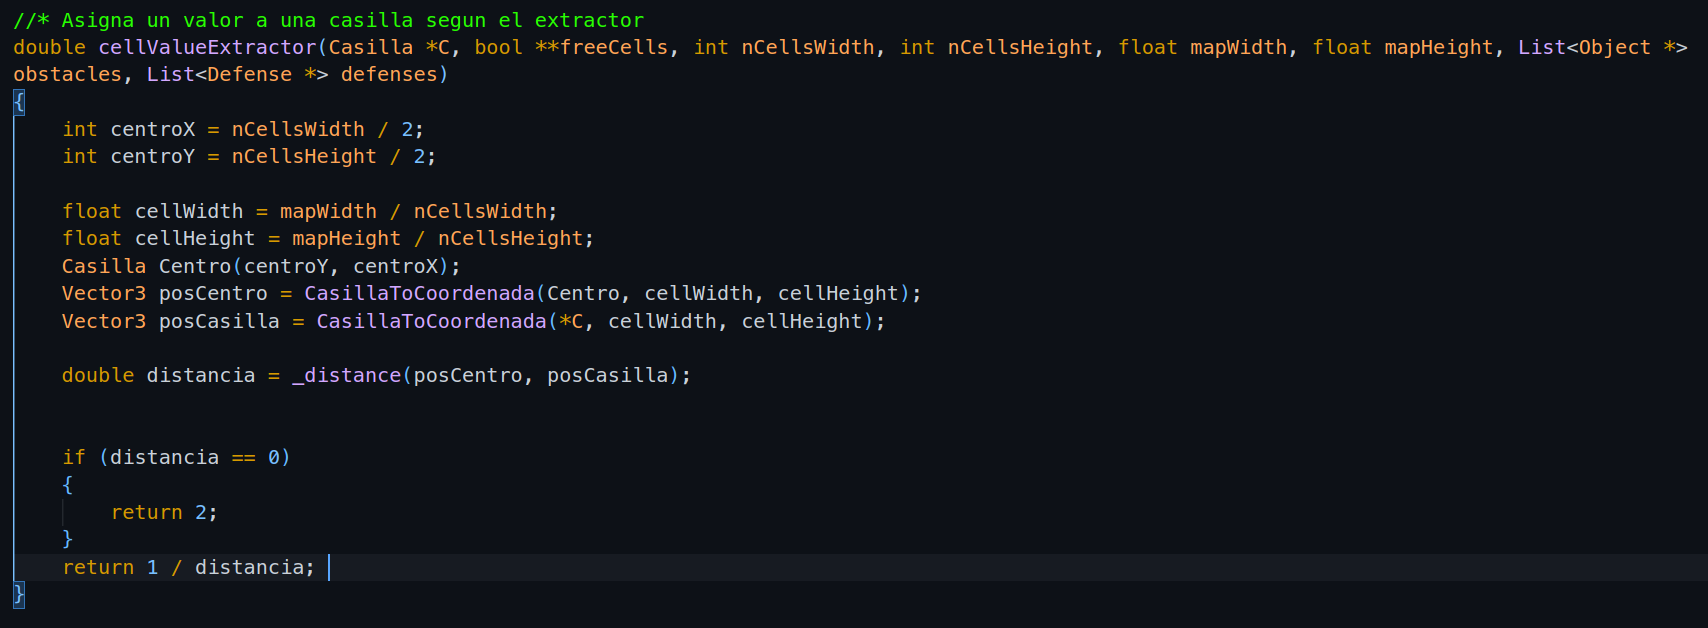
\includegraphics[width=0.7\linewidth]{./CellValueExtractor.png} % no es necesario especificar la extensión del archivo que contiene la imagen
\caption{Estrategia devoradora para la mina}
\label{fig:defenseValueCellsHead}
\end{figure}

\item Incluya a continuación el código fuente relevante del algoritmo.

\begin{lstlisting}
void ordenacionInsercion(int *v, int i, int j)
{
    int aux = 0;
    int k;
    for (int l = i + 1; l <= j; l++)
    {
        bool colocado = false;
        int m = l;
        for (k = l - 1; k >= i && !colocado; k--)
        {
            if (v[m] > v[k])
            {
                aux = v[k];
                v[k] = v[m];
                v[m] = aux;
                m--;
            }
        }
    }
}
void fusion(int *v, int *w, int i, int k, int j)
{
    int n = j - i + 1;
    int p = i;
    int q = k + 1;
    for (int l = 0; l < n; l++)
    {
        if (p <= k && (q > j || v[p] > v[q]))
        {
            w[l] = v[p];
            p = p + 1;
        }
        else
        {
            w[l] = v[q];
            q = q + 1;
        }
    }

    for (int l = 0; l < n; l++)
    {
        v[i + l] = w[l];
    }
}
void ordenacionFusion(int *v, int *w, int i, int j)
{
    int n = j - i + 1;
    if (n <= 3)
    {
        ordenacionInsercion(v, i, j);
    }
    else
    {
        int k = i - 1 + n / 2;
        ordenacionFusion(v, w, i, k);
        ordenacionFusion(v, w, k + 1, j);
        fusion(v, w, i, k, j);
    }
}


void ordenacionRapida(int *v, int i, int j)
{
    int n = j - i + 1;
    if (n <= 3)
    {
        ordenacionInsercion(v, i, j);
    }
    else
    {
        int p = pivote(v, i, j);
        ordenacionRapida(v, i, p - 1);
        ordenacionRapida(v, p + 1, j);
    }
}

\end{lstlisting}


\end{enumerate}

Todo el material incluido en esta memoria y en los ficheros asociados es de mi autoría o ha sido facilitado por los profesores de la asignatura. Haciendo entrega de esta práctica confirmo que he leído la normativa de la asignatura, incluido el punto que respecta al uso de material no original.

\end{document}
